% ==============================================================================
% PG - Nome do Aluno
% Capítulo 3 - Contribuição
% ==============================================================================
\chapter{Contribuição do Trabalho}
\label{sec-contribuicao}

% Este capítulo deve apresentar a principal contribuição do trabalho. Caso o aluno e orientador desejem, o título do capítulo pode ser alterado para referenciar diretamente a contribuição (por exemplo, PIS: Plataforma para Integração de Serviços; Um Sistema para Controle de Processos da UFES, Solução de Otimização para Carregamento de Contêineres; etc.)

% O capítulo deve ser estruturado em seções de forma a apresentar de forma clara e com todas as informações necessárias, a contribuição do trabalho. Por exemplo, caso a contribuição produzida seja um sistema de informação, espera-se que sejam apresentados seus requisitos, funcionalidades, modelos (p.ex., modelo estrutural, modelo da arquitetura, etc.) e telas do sistema. Caso seja uma plataforma, espera-se que a plataforma como um todo seja apresentada e que seus componentes sejam descritos sejam apropriadamente.

Este capítulo tem o propósito de detalhar o escopo da Super Labes World, aplicando os conceitos de engenharia de software para identificar seus requisitos para então construir modelos de casos de uso e diagramas de classe. Na seção \ref{sec:descricao-do-cenario} fazemos uma breve explicação do cenário que foi incentivo para a criação desse trabalho, a seção \ref{sec:escopo} descreve o o intuito desse trabalho, na seção\ref{sec:jogo} é ,  , na seção \ref{sec:usuarios} é descrito quem são os possíveis usuários desse software \ref{sec:diagrama-de-classes}
\section{Descrição do Cenário}
\label{sec:descricao-do-cenario}
Alice uma estudante hipotética recém-chegada ao curso de ciência da computação na UFES sonhava em participar de projetos práticos que envolvessem programação e inovação e que fizessem diferença na sociedade. Com isso em mente, ela decide se candidatar ao LabES, um laboratório de extensão da UFES. Pouco tempo após preencher o formulário no site ela é contactada pela equipe responsável pelo embarque e rapidamente entra em um dos projetos.

Ao começar no projeto ela percebe que é a mais nova dentre os membros e não entende alguns termos utilizados e ferramentas utilizados entre eles. Bob que é o membro sênior,  junto aos demais estudantes estão repletos de atividades e não consegue dar atenção inicial necessária a Alice. Mas ela é uma estudante dedicada e persegue os seus objetivos, então ela elaborou um plano de estudos e o aplicava durante as noites. Após algumas semanas após começou a dar bons resultados no projeto.

Nesse processo que ocorre diariamente em vários laboratórios da UFES alguns dos estudantes desistem no meio do caminho. Nem todos os estudantes são autodidata e persistem como Alice, alguns desanimam no meio do caminho. Esse é um problema complexo que não existe um único culpado nem um único ponto a ser resolvido. 

\section{Escopo}
\label{sec:escopo}
Diante da situação descrita na seção \ref{sec:descricao-do-cenario} surge a ideia de ciar o Super Labes World um RPG desktop desenvolvido com o intuito de ser uma ferramenta lúdica e didática, que possa ser utilizada no auxilio de estudantes para testar, reforçar e adquirir novos conhecimentos. Em sua versão inicial focada aos estudantes do LabES, porém que possa futuramente ser estendido para outros laboratórios e áreas da UFES.

\section{O Jogo}
\label{sec:jogo}
A ambientação do \textit{game} se passa na UFES, o personagem começa acordando em sua casa e lembra que que tem que realizar um teste para entrar no SigAMAES. Durante a exploração inicial e interação com personagens, o jogador é dirigido ao ct7, onde estão localizados os professores e assim pode "batalhar" com os professores, que são os chefes a serem vencidos. A batalha é no estilo perguntas e respostas sendo que o jogador tem quatro opções para escolher. O tema das questões depende de cada professor, que são mestres em disciplinas específicas.
\begin{itemize}
    \item \textbf{Professor Vitor: }contém perguntas relacionadas a área de programação em java e conceitos de docker;
    \item \textbf{Professor Monalessa: }contém questões atreladas a git, gitlab e gitflow;
    \item \textbf{Professor Patrícia: } contém as questões que vão de encontro a metodologia do LabES
\end{itemize}
Ao final da batalha caso o jogador vença, o professor entrega sua chave, representando a sua aprovação nesta disciplina. Somando as três chaves o jogador pode finalmente ter acesso ao LabES.
Caso o jogador erre mais do que 30\% das perguntas a batalha é finalizada, e o professor o instrui a utilizar o computador. 

O computador é uma mecânica do jogo que pode ser acessada a partir dos mapas ''sala do professor'' e ''labgrad''.  Essa interface contém os \textit{links} para materiais de estudos abordados nas questões que o jogador errou. Ao clicar nesse \textit{link} ele será redirecionado a esse conteúdo onde o aluno poderá aprender e tentar passar de nível de novo.
\subsection{Usuários}
\label{sec:usuarios}
O Super Labes World é uma versão inicial de um jogo que tem potencial de ser muito extensível, durante a elaboração do projeto foram identificados três potenciais usuários que podem ser usuário desse trabalho.

\begin{enumerate}
    \item \textbf{Estudantes da UFES que desejam iniciar LabES:} O principal usuário do Super Labes World são estudantes da UFES que desejam iniciar ou são iniciantes no LabES, toda a história do jogo, musicas, efeitos sonoros, interface, items, questões, diálogos de personagens e personagens foram criados com isso em mente, de forma que o jogador possa se identificar e manter-se engajado no game. 
    \item \textbf{Professores:} Um outro possível usuário do jogo são professores que podem alterar as perguntas e recriar o jogo, para diferentes propósitos. 
    \item \textbf{Estudantes de computação:} O jogo pode ser interessante para qualquer estudante de computação, uma vez que trata de questões da área.
\end{enumerate}

\begin{landscape}
\section{Diagrama de Classes}
\label{sec:diagrama-de-classes}
% tabela com as classes
Um Diagrama de classes UML (Unified Modeling Language) Linguagem de Modelagem Unificada é uma notação gráfica para modelagem de software. Essa linguagem define um conjunto de diagramas para documentar e ajudar no design de sistemas de software, particularmente sistemas orientados a objetos \cite{engsoftmoderna}. Esse tipo de modelagem e muito útil durante todo o desenvolvimento do sistema, porque auxilia os desenvolvedores a estruturar o sistema, identificar requisitos e remover os que não forem realmente necessários e ajudando na comunicação entre a equipe.

Para detalhar melhor cada uma das classes apresentadas, no diagrama \ref{fig:diagrama-de-classes-uml} foi elaborada o diagrama de classes UML afim de representar modelos de dados para sistemas de devido software e assim compreender de forma mais ampla a visão geral do trabalho. O resultado pode ser visualizado a seguir na figura \ref{fig:diagrama-de-classes-uml}
seguir. 
\begin{figure}[h!]
    \centering
    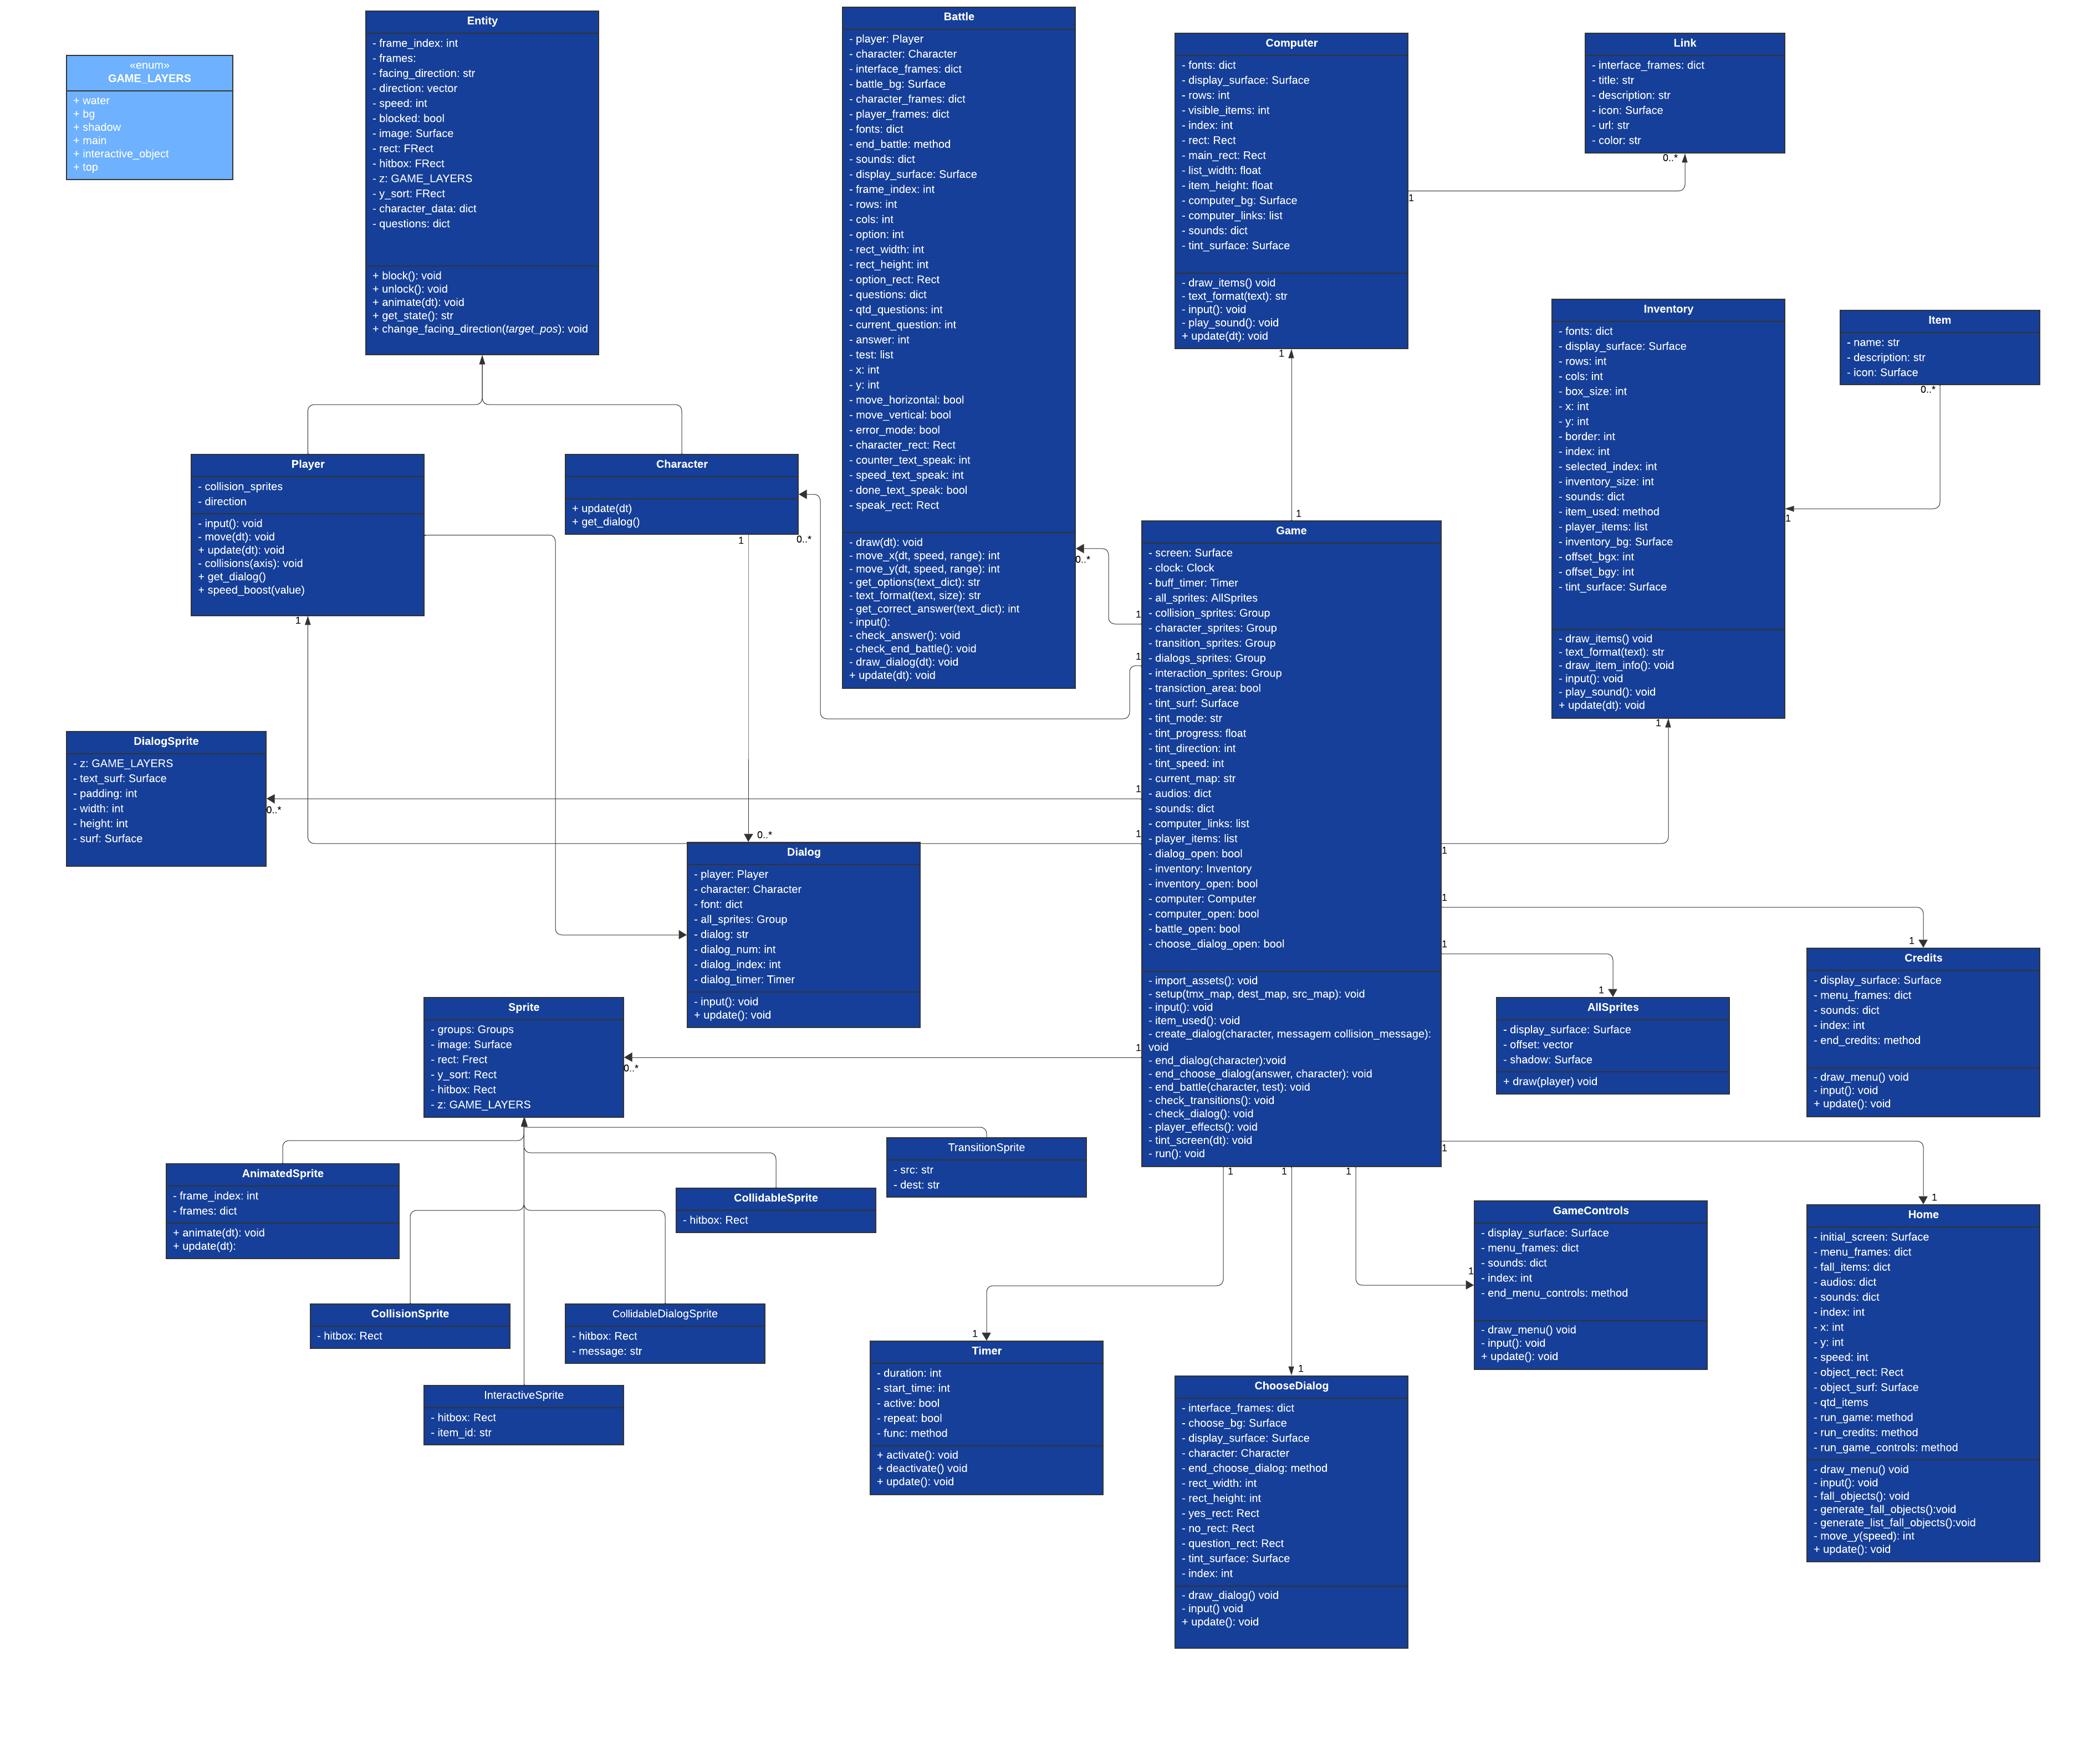
\includegraphics[width=0.8\linewidth]{figuras/diagrama-de-classes-uml.png}
    \caption{Diagrama de Classes do Super Labes World}
    \label{fig:diagrama-de-classes-uml}
\end{figure}
\end{landscape}

Para especificar o diagrama anterior, foi criada uma tabela descrevendo as classes e sua função principal que podem ser vistas nas tabelas \ref{tbl-especificacao-classes-1}, \ref{tbl-especificacao-classes-2} e \ref{tbl-especificacao-classes-3}.

\begin{table}[h!]
	\caption{Tabela especificando as classes do Super Labes World.}
	\label{tbl-especificacao-classes-1}
	\centering
	\renewcommand{\arraystretch}{2}
	\begin{small}
		\begin{tabular}{ | p{35mm} | p{100mm} |}\hline \rowcolor{MidnightBlue}
			\centering{\textbf{Classe}} & \textbf{Descrição}  \\\hline		
			\centering{\textit{AllSprites}} & Classe responsável por representar a câmera do jogador. \\\hline
			\centering{\textit{Entity}} & Classe Pai que contém informações comuns a todas as entidades do jogo como frames, \textit{hitbox} e métodos relacionados a animação.   \\\hline
			\centering{\textit{Player}} & Classe filho de \textit{Entity}, configura atributos inerentes ao jogador como movimentação, colisão, e modificações de seus atributos.  \\\hline
			\centering{\textit{Character}} & Classe que herda \textit{Entity} sua principal característica é o método de obtenção de diálogo relativo ao personagem.\\\hline
			\centering{\textit{Battle}} & Classe que contém todas as informações que fazer parte da batalha do jogo, destacando \textit{questions} que contém as questões relativas ao personagem em batalha e \textit{test} que é uma lista que armazena 0 para respostas erradas e 1 para respostas corretas.\\\hline
			\centering{\textit{Computer}} & Classe responsável pela tela de visualização do computador, sua maior peculiaridade é o atributo \textit{computer\_links} que mantém um \textit{array} de \textit{Items} que serão mostrados ao entrar nessa tela. \\\hline
			\centering{\textit{Link}} & Contém informações que serão mostradas no computador como título, descrição, url a ser redirecionada, cor e icon que deve ser uma imagem 108 x 108 \\\hline
			\centering{\textit{Game}} & Classe principal do jogo, contém o main loop é responsável por carregar todos os \textit{assets} e capturar todo o I/O do jogador. \\\hline
			\centering{\textit{Inventory}} & Classe utilizada para representação visual do inventário do jogador. \\\hline
			\centering{Item} & Classe que armazena informações do item (nome, descrição e ícone) o tamanho ícone deve ser 93 x 93 \\\hline
		\end{tabular}
	\end{small}
\end{table}

\begin{table}[h!]
	\caption{Tabela com a continuação da especificação de classes do Super Labes World.}
	\label{tbl-especificacao-classes-2}
	\centering
	\renewcommand{\arraystretch}{2}
	\begin{small}
		\begin{tabular}{ | p{35mm} | p{100mm} |}\hline \rowcolor{MidnightBlue}
			  \centering{\textbf{Classe}} & \textbf{Descrição}  \\\hline
			\centering{\textit{DialogSprite}} & Classe que realiza o desenho do diálogo na tela. \\\hline
			\centering{\textit{CollisionSprite}} & Classe que contém as informações da sua classe pai \textit{Sprite}, sua singularidade é ter uma \textit{hitbox}\\\hline
			\centering{\textit{CollidableSprite}} & Classe que herda os atributos de \textit{Sprite}, oque o difere de CollisionSprite é a área de colisão desses sprites é menor.  \\\hline
			\centering{\textit{InteractiveSprite}} & Classe que herda a classe pai \textit{Sprite}, sua peculiaridade é ter uma variável item\_id que da liberdade ao programador para definir qual ação será realizada a partir de uma interação do jogador. \\\hline
			\centering{\textit{CollidableDialogSprite}} & Classe que herda \textit{Sprite}, a sua característica que diferencia das outras é não ter uma imagem associada e armazenar uma mensagem  que ao player colidir é lançada na tela. \\\hline
			\centering{\textit{AnimatedSprite}} & Classe filho de \textit{Sprite} contém todos os \textit{sprites} que são animados automaticamente  \\\hline
			\centering{\textit{TransitionSprite}} & Classe que herda \textit{Sprite}, sua principal característa é que ela guarda informações de origem e destino para poder realizar as transições de forma correta. \\\hline
			\centering{\textit{ChooseDialog}} & Classe que representa o diálogo de escolha do jogador antes de entrar em uma batalha. \\\hline
			\centering{\textit{Dialog}} & Classe responsável por criar os diálogos de todos os personagens do jogo. \\\hline
			\centering{\textit{Sprite}} & Classe Pai de todas os tipos de sprites do jogo, suas informações mais importantes são a imagem que representa o sprite, a sua posição e em qual camada ele está. \\\hline
			\centering{\textit{Timer}} & Classe que é responsável por realizar os controles de tempo do jogo.  \\\hline
		\end{tabular}
	\end{small}
\end{table}

\begin{table}[t]
	\caption{Tabela com a continuação da especificação de classes do Super Labes World.}
	\label{tbl-especificacao-classes-3}
	\centering
	\renewcommand{\arraystretch}{2}
	\begin{small}
		\begin{tabular}{ | p{35mm} | p{100mm} |}\hline \rowcolor{MidnightBlue}
			  \centering{\textbf{Classe}} & \textbf{Descrição}  \\\hline
			\centering{\textit{Home}} & Classe que representa o menu inicial. \\\hline
			\centering{\textit{GameControls}} & Classe que representa a tela de controles que pode ser acessada apenas da tela inicial. \\\hline
			\centering{\textit{Credits}} & Classe que representa a tela de créditos que apenas pode ser acessada da tela inicial.\\\hline
		\end{tabular}
	\end{small}
\end{table}
\clearpage
\section{Conclusões do Capítulo}
\label{sec:conclusoes-do-capitulo-3}
Este capítulo apresentou diversos aspectos essenciais para o desenvolvimento do sistema. Inicialmente, foi estabelecido o minimundo que foi o motivador para criação desse trabalho, nele é fornecido uma descrição clara e objetiva do contexto em que o sistema está inserido. Essa definição facilita a compreensão dos desafios e metas a serem atingidos.

Com isso foi possível definir o escopo que esse trabalho se propõe a atingir, bem como a história do jogo e as suas principais mecânicas.  

Por fim foi apresentado o diagrama de classes, que desempenha um papel essencial na definição da estrutura do sistema. Com esse diagrama, foram identificadas as classes que representam os elementos do sistema e as relações entre elas. Esse diagrama junto a tabela de especificação de classes ajudaram na representação visual e facilitaram a compreensão das entidades do sistema e suas interações, auxiliando no planejamento para a implementação do sistema.

